%$Id$
\documentclass[conference, compsoc]{IEEEtran}
\usepackage{fontspec}
%\usepackage{amsmath,amssymb,amsthm,supertabular,booktabs,rotating,semantic,subfigure,multirow,colortbl}
\usepackage{graphicx, url}
\usepackage[colorlinks=true,linkcolor=black,anchorcolor=black,citecolor=black,urlcolor=black,bookmarks=false,pdfstartview=FitH]{hyperref}
\usepackage{algorithmic}
\usepackage{xunicode}
\usepackage{xltxtra}
\defaultfontfeatures{Mapping=tex-text}
\setmainfont{Times New Roman}
\begin{document}

\bibliographystyle{IEEEtran}
 
\title{Understanding software quality evolution using signifier frequency extraction}
\author{
Neil A. Ernst\\Dept. of Computer Science\\University of Toronto\\nernst@cs.toronto.edu \and
John Mylopoulos\\Dept. of Computer Science\\University of Toronto\\jm@cs.toronto.edu }

\maketitle

\begin{abstract}
We describe a repository mining technique we call signifier extraction. We generate signifiers using Wordnet and the ISO quality taxonomy. Using corpora created from eight Gnome projects -- their mailing lists, subversion comments, and bug comments -- we search for the signifiers over three month, quarterly intervals. The occurrence of our signifiers forms an evolutionary pattern that we analyze statistically and historically. We show that it is possible to reconstruct the historical evolution of project responses to external forcings, such as release cycles and audits. [numbers?]
\end{abstract}

\section{Introduction}\label{sect:introduction}%Aim
\begin{quote}[My impression] is of a large project in a state of marginal returns, in which a larger and larger part of the effort goes to maintenance. -- Andy Wingo, Gnome developer, June 2008.\footnote{http://wingolog.org/archives/2008/06/07/gnome-in-the-age-of-decadence}\end{quote}
	This quote, from a participant in the Gnome ecosystem (a developer), captures some of what this paper tries to elucidate. Is it the case that as projects mature the focus and effort of the developers turns to maintenance tasks? \cite{swanson} Certainly Lehman's conclusions \cite{lehman} is that this is the case (viz. Lehman's 2nd `law'). Can we demonstrate this empirically? To test this notion, we begin with a few assumptions. The first requirement we have is for some sort of signal we can capture that will signify that `maintenance' is being done. One approach is to scan code for maintenance activity, like the work of [who]. Our approach is focused on the conversations developers have (with each other or with `users') [refer to various players in OSS -- Scacchi?]. To identify when `effort goes to maintenance', we assume that a discussion that uses some signifiers for various maintenance properties -- defined as ISO9126 software quality model [not really maintenance, maintenance is more like bug fixes and incrementalism]
	
\begin{figure}[b]
\centering
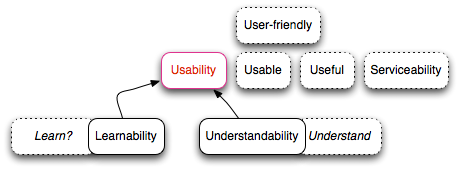
\includegraphics[width=0.4\textwidth]{synonym-graph.png}
\caption{An extensional definition of usability}
\label{fig:syngraph}
\end{figure}
	
	
\section{Signifier extraction} %Method
In semiotics, Peirce first made the distinction drawn between signifier, signified, and sign~\cite{atkin2006}. In this work, we make use of signifiers -- words like `usability' and `usable' -- to capture the occurrence in our corpora of the signified -- in this example, the concept `usability'. We extract our signified, concept words from the ISO 9126 quality model~\cite{iso9126}. There is some debate about the significance and importance of the terms in this model. However, it is ``an international standard and thus provides an internationally accepted terminology for software quality~\cite[p. 58]{Boegh2008},'' which is sufficient for the purposes of this research. The model is used to refer to both external and internal views of quality (for example, bugs filed by users would be external qualities, whereas an email discussion of features to come would be internal). We generate the signifiers from Wordnet~\cite{Fellbaum1998}, an English-language `lexical database' that contains semantic relations between words, including meronymy and synonymy. We extract words using the following criteria: 
\begin{algorithmic}
	\caption{Defining signified terms extensionally}
	\FOR{all top-level terms in ISO9126 model}
	\COMMENT{case-insensitively}
	\STATE define it as a wordnet noun
	\STATE query its synset in wordnet
	\STATE identify its direct h
	\STATE for each sub-term (meronym) in ISO9126 
	\COMMENT a meronym is the sub-part of a greater whole (e.g., partonymy)
	\ENDFOR
	\RETURN the list of `events' per signified term
	
take the term in the ISO9126 model
query it (upper/lower case), in wordnet. Note, we do not currently look for common misspellings or other languages (the primary language is English, at any rate).
for each occurrence, take its uses
add those to the bubble
query corpus for each term in the bubble
	add those events to the overall events for the signified

\end{algorithmic}
These criteria give us a linguistic `bubble' which we use to extensionally define the signified.

\section{Observations}
[The graphs]
\subsection{Discussion}
We include a linear regression of the number of occurrences against the date. The equation of the regression line shows the average value of the number of occurrences as the date increases. A linear relationship may not be a good model of the actual pattern. For example, the number of occurrences may be changing in response to some other variable, such as co-ordinated release dates (plotted as vertical gray lines, above); developer illness, and many others. In many ways this is the purpose of this set of experiments. Nonetheless, one of the key questions this research project initially proposed was `does quality become of greater interest as a project matures', which is shown by the linear regression line. To measure the significance of this relationship, we also measure the squared correlation value, $r^2$, which ranges from 0--1, where 1 indicated perfect correlation.
Multi-level modeling
Set windows at each release to see what is happening prior and after the release (e.g., unit of analysis becomes the release period, not `quarters')
\section{Threats}
missing words and phrases that are related to the signifier but don't contain it (e.g., ``can't find the submit button" vs. ``usability")). 
mentions that aren't related to product
normalize? We don't, because we are interested in absolute numbers. For example, suppose that in the month prior to the release we get a huge spike in mailing list traffic, as the developers work out the features to be frozen. We want to retain the absolute number of events, not relative. Maybe not, maybe we want both.
Some words are not well-defined in general purpose ways like Wordnet or general dictionaries.
Some signified terms are defined by more signifiers, which should skew their occurrence counts.
\section{Future work and conclusions}
[did we see a trend]
[social element: who is doing what, new people come in.. case study?]
\section{Appendix}
Source code, data, and related discussions are available at \url{http://neilernst.net/msr09/}.
\begin{footnotesize}
\bibliography{msr}
\end{footnotesize}
\end{document}



% I suspect the underlying problem you are having is how
% to cope with requirements churn. From Mary Poppendieck's
% book "Implementing Lean Software Development" there's this
% very valuable tip:
% 
% "If you have requirements churn, you are specifying too
% early".